\documentclass{article}
\usepackage[utf8]{inputenc}

\title{Lecture 6: Bayesian inference }
\author{wbg231 }
\date{November 2022}
\usepackage{tikz,graphicx,amsmath,amsfonts,amscd,amssymb,bm,cite,epsfig,epsf,url}
\begin{document}

\maketitle

\section{Introduction}
\subsection{frequentest vs Bayes }
\begin{itemize}
%\item 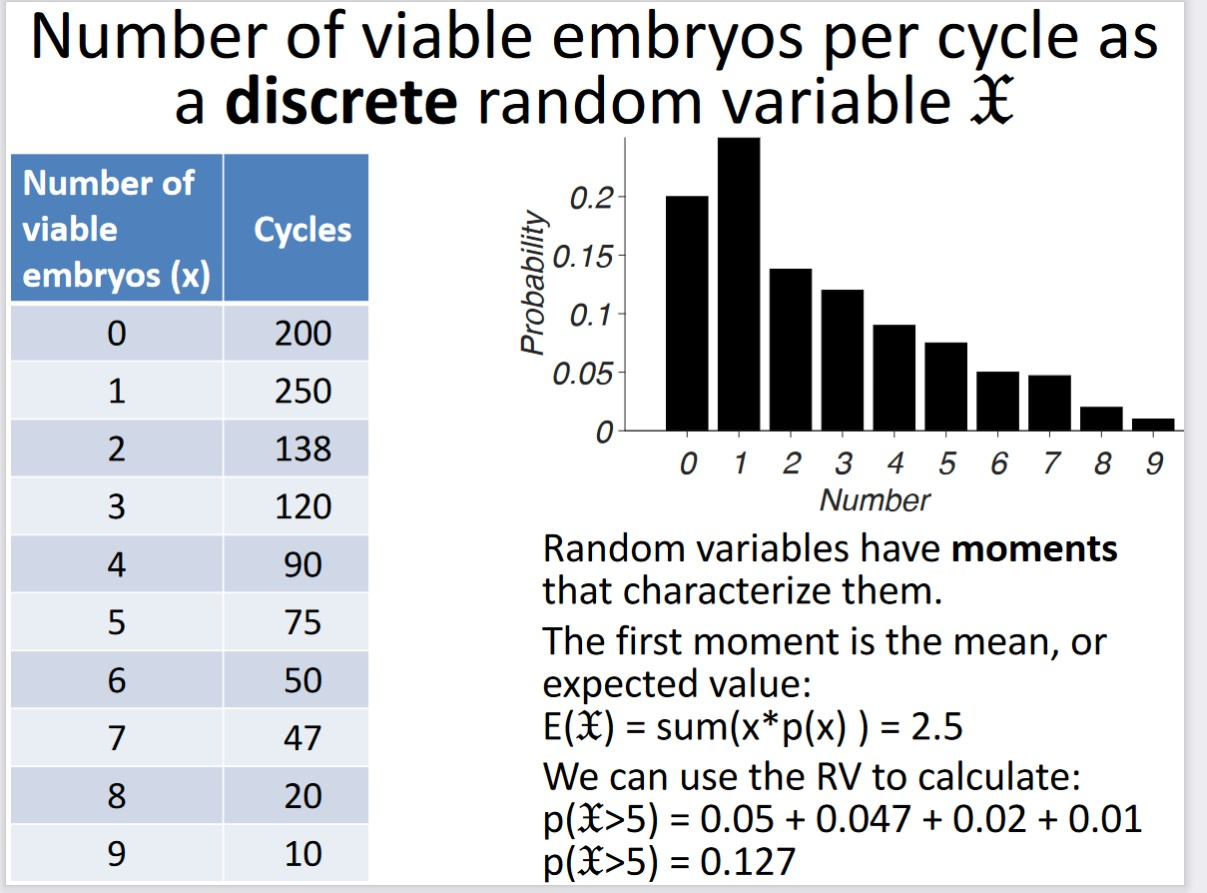
\includegraphics[width=7.5cm]{Final_Review/Lecture_2/lecture_1example.jpg}
\item this is all about parameter estimates instead of just gauging if something is significant
\item in Bayesian what are important are the prior, the likelihood and the posterior
\item the prior and the likelihood are always fighting
\item everything so far is frequentest
\item in the frequentest conceptions relative frequency of the outcome of interest as a proportion of the whole sample space in the long run (objective probability) 
\item but this fails if the system is ergotic 
\item the Bayesian conception: degree of belief are constantly updating with new information (subjective probability)
\subsection{Bayes background}
\item Bayes said that prior information matters
\item 2009 air France flight crashed in the ocean, they wanted to get the black box very quickly, where would you start looking for the plane?
\item where you last saw it so your prior matters
\item they instead did a grid search of the whole credible area randomly and it took two years. 
\item so taking into account prior information is important 
\subsection{where does Bayes theorem come from }
\item Bayes worked this out on the back of a piece of paper, and never published it. 
\item Bayesian statistics are increasingly important, it is likely this will be how we deal with probability in the future 
\item this is working with conditional probabilities updates and inverts them.
\item the brain is a Bayesian machine. 
\item the idea is: data does not speak for its self, evidence just updates the prior beliefs. 
\item fisher thought that was a bug, Bayes thought that was a feature.
\item fisher thought that frequentest framework was a update or improvement since you do not need a prior. 
\subsection{deriving Bayes theorem }
\item given to events A, B $P(A|B)=\frac{P(A\cap B)}{P(b)}=\frac{P(B|A)P(A))}{P(b)}$
\subsection{terminology}
\item P(A), P(B) are called our priors
\item $P(B|A)$ is our likelihood, this is a conditional probability, it is the one we have not the one we want 
\itme P(A|B) is the posterior, it is the evidence ie what we want 
\subsection{spam filter example}
\item we want to build a spam filter 
\item 1 in 100 massages are spam 
\item all spam messages have a certain key word 
\item 1 in 10 message shave that keyword 
\item would filtering massages with  a certain keyword and flagging them as a spam be a good approach or would we expect to many false positives? 
\item let A be if something is spam, b be if it contains a keyword. 
\item$ P(A)=\frac{1}{10} P(B)=\frac{1}{100} P(B|A)=1$
\item so$ P(a|b)=\frac{\frac{1}{100}}{\frac{1}{10}}=\frac{1}{10}$ so it is not a good idea to just call everything with that keyword spam. since you would have 90\% false positives
\section{on priors}
\subsection{ the prior vs the likelihood}
\item say that spam is becoming more common $P(B)=\frac{1}{20}$ this tells us that $P(A|b)=\frac{\frac{1}{20}}{\frac{1}{10}}=\frac{10}{20}=.5$
\item so the point is the prior probability of spam has become more common 
\item if people stop using these keywords then our posterior changes again. 
\item the challenge again is to well define our prior. 
\section{Bayesian statistical inference}
\item null hypothesis significance testing has a convoluted logic.
\item it also only tells us if there is significance not how much 
\item the Bayes factor provides an alternative approach. it is the Bayesian version of a p-value 
\item they were specifically designed to address the questions of, what is the likely effect, and what is the likelihood of our hypothesis being true given the data, as opposed to what is the likely hood of our data given our hypothesis is false.
\subsection{Bayes factor}
\item we can express our posterior odds as $\frac{P(h_1|D)}{P(h_0|D)}=\frac{P(D|h_1)}{P(D|h_0)}*\frac{P(h_1)}{P(h_0)}$ we can also sometimes write this in the explicit from as $\frac{P(h_1|D)}{P(h_0|D)}=\frac{P(D|h_1)}{P(D|h_0)}*\frac{P(h_1)}{P(h_0)}=\frac{P(D|H_1)(P(h_0|d)P(h_0)+P(H_0^c)P(d|H_0^c))}{P(D|H_1\0)(P(h_1|d)P(h_1)+P(H_1^c)P(d|H_1^c))}\frac{P(h_1)}{P(h_0)}$ using the law of total probability
\item it can just be computed using Bayes rule
\item $H_1$ is the event the data is true.
\item $\frac{P(h_1)}{P(h_0)}$ are our prior odds
\item $\frac{P(H_1|D)}{P(H_0|D)}$ there are our posterior odds
\item $\frac{P(D|H_1)(P(h_0|d)P(h_0)+P(H_0^c)P(d|H_0^c))}{P(D|H_1\0)(P(h_1|d)P(h_1)+P(H_1^c)P(d|H_1^c))}$ this is called our likelihood diferential
\item the Bayes factor is $\frac{P(D|h_1)}{P(D|h_0)}$
\item what have we already seen? the denominator of the Bayes factor! $P(D|h_0)$ are the classic p value 
\item so in other words Bayes factors contextualize the p values
\item in an ideal world we want the posterior odds$\frac{P(H_1|D)}{P(H_0|D)}$
\item but in reality we do not usually have access to $\frac{P(h_1)}{P(h_0)}$  our prior odds, so we usually just report the Bayes factor
\item in Bayesian inference we usually stop at the Bayes factor but that is usually OK. 
\item Bayes factor$ bf=\frac{P(D|h_1)}{P(D|H_0)}$ these were introduced in the 1930s but ignored 
\subsection{what do Bayes factors get us }
\item Bayes factor$ bf=\frac{P(D|h_1)}{P(D|H_0)}$ allow us to quantify the strength in factor of a hypothesis. 
\item is the data more liekly assuming the null or the alternative
\item there is a problem with bayes factors however? 
\item  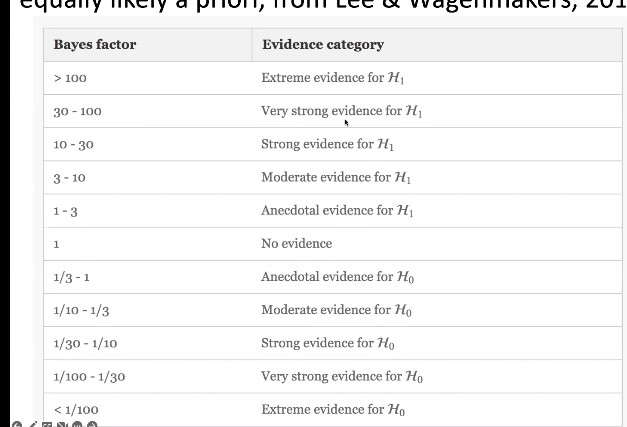
\includegraphics[width=7.5cm]{Final_Review/lecture_6/bayes factor table.jpg}
\item there is not a standard agreed upon cut off for Bayes factor equivalent to $\alpha=.05$ there is no clear threshold to reject the null
\subsection{calculating the numerator}
\item how do we calculate the numerator ie $P(d|h_1)$
\item  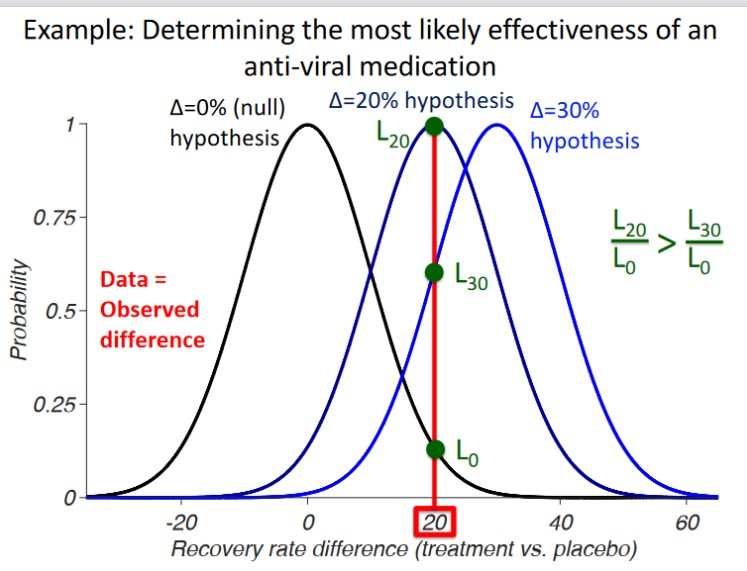
\includegraphics[width=10cm]{Final_Review/lecture_6/virus example.jpg}
\item example everyone has some virus we want to see how people with the virus react to a treatment
\item think of these curves as the distribution of a random variable representing the mean difference between two samples (one treated one untreated) call it $\Delta$
\item the furthest to the left curve is the distribution if our null hypothesis is true that is $\Delta=0$ 
\item the other two curves represent different alternative hypothesis, 
\item so suppose in the data we really saw that the recovery rate difference was 20 ie at that red line. 
\item then $L_20$ is the likelihood under the 20 hypothesis that is $P(D|H_{20})$ it is a conditional likelihood
\item $L-0$ is the likelihood of observing the data assuming it came from the null $L_0=P(D|h_{0})$
\item so from this we can conclude that $\frac{l_{20}}{L{0}}>\frac{l_{30}}{L_{0}}$ that is given the data the 20 hypothesis is more likely than the 30 hypothesis 
\item $L_20, L_30$ are not special we can consider any alternatives we want. 
\item that is the idea given the data which distribution is more likely if we assume some distribution? 
\subsection{Bayesian stats can help access the replicability  crisis }
\item what is the probability that a published result is actually true?
\item if we set the significance level $\alpha=.05$ does this mean that the false positive rate of a significant results is 5\%? no this is false 
\item it also depends on the prior probability of a true effect given the field as well as the statistical power
\item so the false positive rate is also determined by our priors as well as power
\section{PPV}
\subsection{PPV}
\item PPV (positive predictive Value) is the post study probability that a significant result is actually true!
\item so PPV is given a result is significant what is the chance it is true 
\item $\textbf{PPV}=\frac{R(1-\beta)}{r-\beta *r +\alpha}=\frac{R(1-\beta)}{(1-\beta)R+\alpha}$
\item $1-\beta$ is power 
\item $\alpha$ is significance level
\item R is the ratio of true to false positive effects in a field 
\item PPC links power alpha and R 
\item here is the derivation of PPV
\item 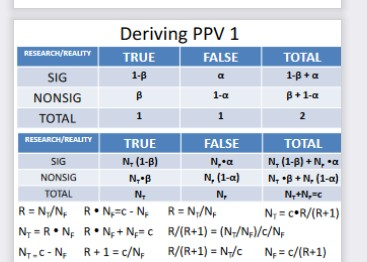
\includegraphics[width=7.5cm]{Final_Review/lecture_6/ppv derivation 1.jpg}
\item 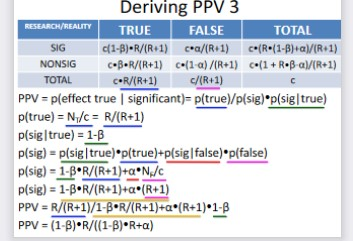
\includegraphics[width=7.5cm]{Final_Review/lecture_6/ppv devation 3.jpg}
\item 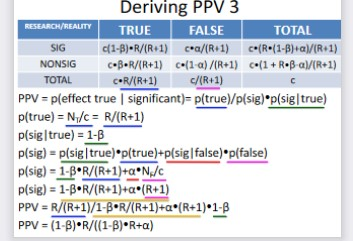
\includegraphics[width=7.5cm]{Final_Review/lecture_6/ppv devation 3.jpg}
\item the work is kind of tedious, the first part is just a confusion matrix. the second part we multiply the false col by the number of false row, and trues by the number of trues.this allows us to express this matrix in terms of the total number of times we see an outcome instead of its probability
\item then step 3 allows us to re-express this in terms of probability this time however (using the number of number of trues and false) 
\item then we just solve for PPV in these terms 
\item we solve for ppv using Bayes. PPV is just $PPV=P(t=1|s=1)=\frac{P(t=1)P(s=1|t=1)}{P(s=1)}$
\subsection{ppv in context of the confusion matrix}
\item 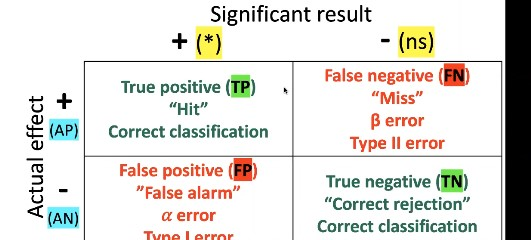
\includegraphics[width=7.5cm]{Final_Review/lecture_6/sigfgence_Test_confusion_matrix.jpg}
\item we can see a confusion matrix here in terms of a significance test 
\item true positive there is an effect and we find it. (also called correct classification or hit
\item if there is  a real effect and we fail to find it that is a type II error or your beta error 
\item if there is no real effect but we find one that is a type one or $\alpha$ error
\item the finally we have a true negative, or a correct rejection, or a correct classification 
\item Prevalence = $\frac{TP+FP}{TP+FP+TN+FN}$ ie the number of positives over everything else
\item accuracy= $f\frac{TP+TN}{TP+TN+FP+FN}$ the number of units that we classify correctly over all individuals, the number of correct judgments
\item sensitivity=$\frac{TP}{TP+FN}$ ie that is the number of things we classify correctly as positive over the the true number of positives. also called recall, power or true positive rate
\item specificity $=\frac{tN}{AN+FP}$ the number of things we classify as negative correctly, over the number of things that should have been classed as negative also called true negative rate
\item what is the fraction of true positives? precision=$\frac{TP}{TP+FP}$ that is how many of the things we classified as true were in fact true that is our PPV
\item these are critical metrics for machine learning 
\subsection{the role of a study}
\item a baysian study takes the prior odds of the effect being true $r=\frac{TP}{TN}=\frac{P(h_1)}{P(h_0)}$ into the posterior-ppv (that is the ppv given the data) as a function of statistical power $1-\beta$ 
\item  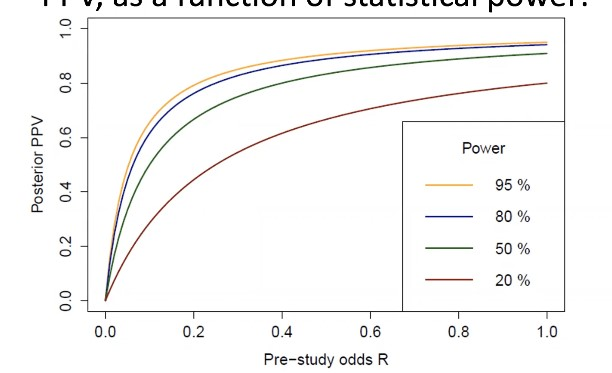
\includegraphics[width=10cm]{Final_Review/lecture_6/ppv_versus_power.jpg}
\item so look at this graph. 
\item x axis is the proportion of true positives, over the number of positives so this is what we care about over a whole field 
\item so this depends on r and power
\item power is most important wehn we have low pre study odds. 
\item the pre study odds of people listing to music and remembering that song better are fairly high, so need a fairly low power to to get a high ppv
\item but if our pre studio prior is low, then with a low of power we can still ensure that we are getting good ppv.
\item so in most research that is being done right now, we are looking for things with low posterior odds with low power studies, so we will have a low ppv, meaning many false positives will be published.
\item so if you have to study things with low pre study odds have really high power. 
\item so this ties power ppv and Bayes. 
\section{Credible intervals}
\subsection{frequentest confidence interval }
\item in the frequentest approach the value of our population parameter $\theta$ is fixed but unknown. we try to estimate it by taking a sample form the population yielding a distribution of sample means which we use to form the confidence interval
\item example you are trying to find the prevalence of a virus in a population by the frequentest approach
\item we estimate a confidence interval and argue that our $\theta$ is within that 

\subsection{Bayesian  primors}
\item in the Bayesian framework our population parameter $\theta$ is a random variable and has a probability distribution 
\item the distribution of $\theta$ corresponds to our degree of belief. 
\item tour prior belief about the value of the parameter is called the prior distribution 
\item the prior can take any shape but the sharper (more strongly held it is) the more informative it is. 
\item often to model the prior distribution of a proportion we use the beta distribution
\item so in Bayesian analysis we use the data from our study, in combination with the prior distribution to compute the posterior distribution 
\item posterior = prior * likelihood that is $P(\theta|y)=P(\theta)P(y|\theta)$ where y is our data 
\subsection{example}
\item suppose we have a somewhat informative prior say a beta distribution with $\alpha=10, \beta=10$
\item the prior has to have come form somewhere but lets say we have it 
\item we take a sample of 100 people and see how many are infected with the virus yielding our data y
\item this yields our posterior $P(\theta|y)$
\item this works alliteratively ie our posterior will become the prior of the next person researching this question
\item
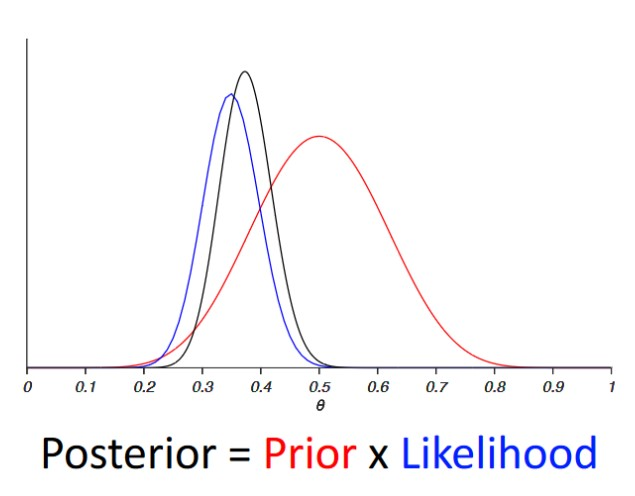
\includegraphics[width=7.5cm]{Final_Review/lecture_6/posteriro=.jpg}
\item so notice that the posterior is a mixture of our prior and likelihood 
\item the credible interval is the area under the posterior bounded by the prior and likelihood
\section{reconciling frequentest and Bayesian ideas}
\subsection{when prior matters}
\item at a small sample size prior has a really big effect.
\item at a large sample size the prior does not matter that much 
\itme in this case the posterior gets a lot tighter, if we have a higher sample size
\subsection{reconciling Bayes and frequentest}
\item the Bayes and frequentest perspective are exactly the same if the sample size is near infinite
\item this was how Fischer was thinking of his work 

\section{When to use which type of inference}
\item 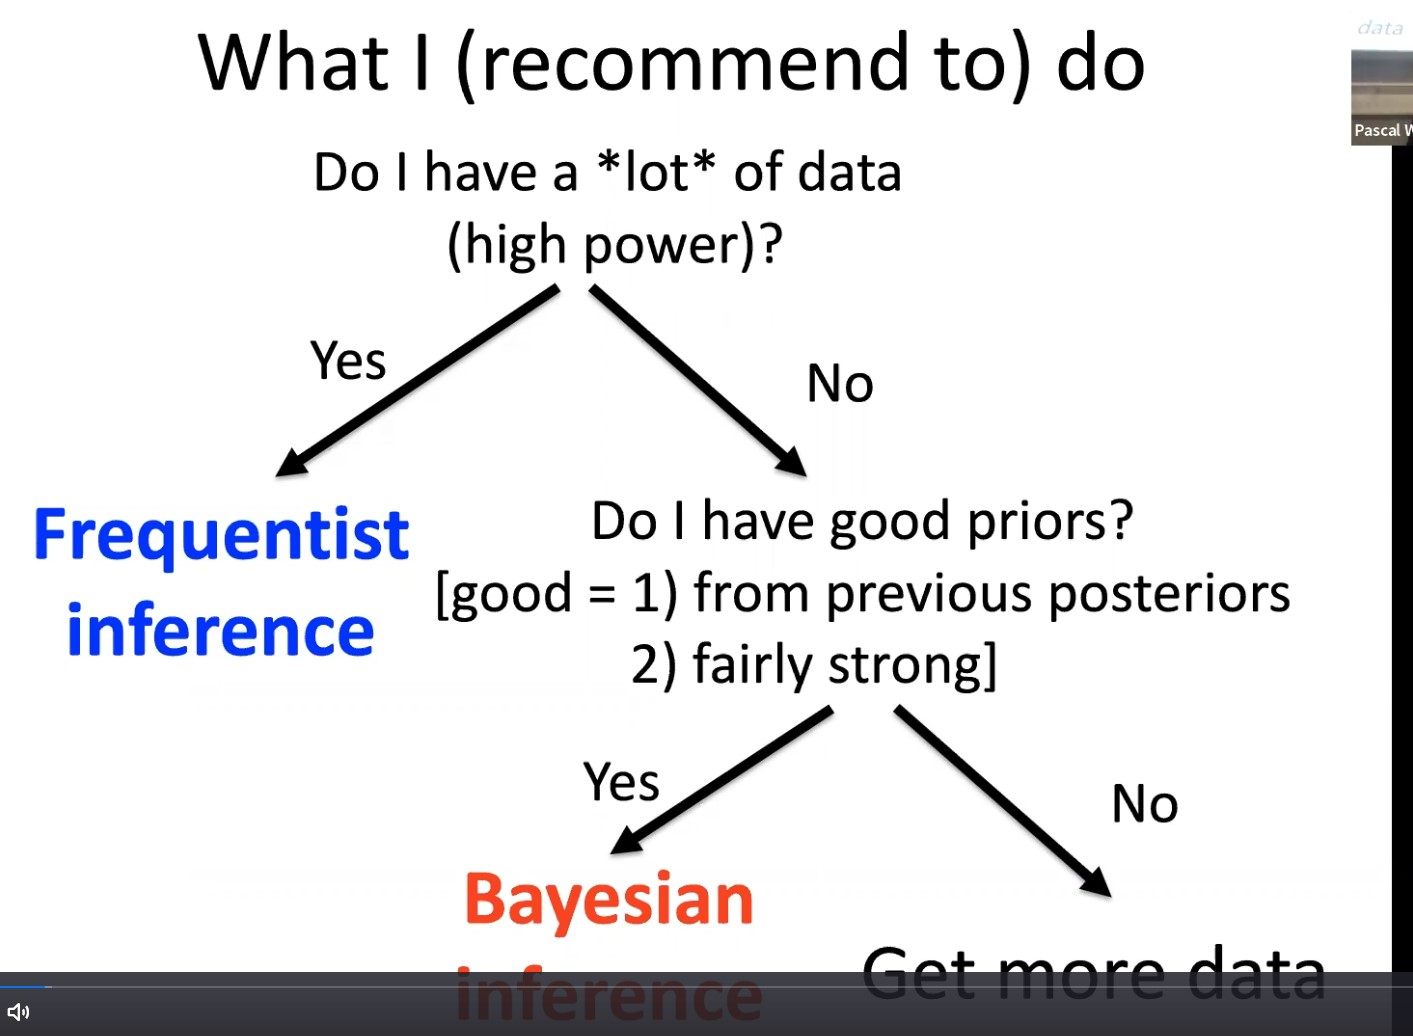
\includegraphics[width=7.5cm]{Final_Review/lecture_6/inference_flow_chart.jpg}

\item  do you have a lot of prior 
\item if yes use frequentest inference 
\item if no ask you self if you have a good prior 
\item if yes the sample size is small and you have good priors then use a Bayesian frame work
\item if you have low data, and no good prior get more data
\item a good prior is a prior that comes from somewhere logical, 
\item you do not need to just pick one and stick with it 


\end{itemize}

\end{document}
